\begin{exmp} 
    Shifted Function: A function viewed in a fixed coordinate $x$ is centered at zero $f(x-0)=f(x)=1+x^2$, 
    and shifted to any center at $x=z$ according to $f(x-z)=1+(x-z)^2$. 
    Therefore the shifted $f(x-z=0)=f(x=z)=1+(z-z)^2=1$ evaluated at the center $x=z$ gives the same function value as the unshifted $f(x=0)=1+x^2=1$ centered at $x=0$.
    Notice the two functions are indistinguishable when given a dummy variable $y=x-z$ and evaluate in separate coordinates, so $f(y)=1+y^2$ is essentially the same as $f(x)$.
    Hence, only if viewed in the same $x$ coordinate will we mention the "shifted function".
\end{exmp}

\begin{exmp} \label{exmp:reflect_func_asym}
    Reflected Function (Asymmetric): A function centered at zero $f(x)=x-1$ being reflected gives $f(-x)=-x-1$, where simply plugging in 
    $x=1$ will give the corresponding function values for the unreflected $f(1)=0$ which is not equal to the reflected $f(-1)=-2$.
    But, the reflected $x=-1$ at $f(-x)$ gives the same function value as $x=1$ at $f(x)$.
\end{exmp}

\begin{exmp}
    Reflected Function (Symmetric): The function centered at zero $f(x)=x^2$ being reflected gives $f(-x)=x^2$ implies $f(x)=f(-x)$.
\end{exmp}

\begin{exmp} \label{exmp:shift_reflect_func_asym}
    Shifted Reflected Function (Asymmetric): $f(x)=x-1 \rightarrow f(2-x)=f(-(x-2))=1-x$ is centered at $x=2$ and reflected (Figure \ref{fig:shift_reflect_func_asym}).
    \begin{figure} [H]
        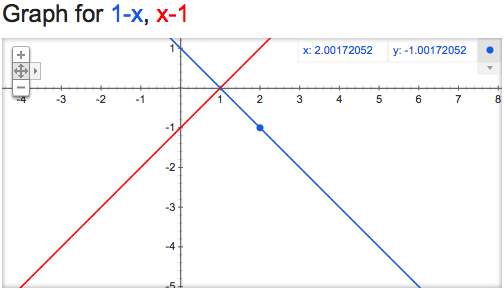
\includegraphics[width=0.6\textwidth]{shift_reflect_func_asym.png}
        \caption{}
        \label{fig:shift_reflect_func_asym}
    \end{figure}
\end{exmp}
